
\documentclass{article}
\usepackage{graphicx} % Required for inserting images
\usepackage[spanish]{babel}
\usepackage{xcolor,colortbl}
\usepackage{graphicx}
\usepackage{amsmath}
\usepackage{tabularx}
\usepackage{booktabs} % Para líneas horizontales más profesionales
\usepackage{array} % Para un mejor control sobre las columnas

\title{Informe de Práctica de Laboratorio IV}
\author{José M. Díaz M. (25.682.785) \and Sergio José Noguera (30.572.211)}
\date{05 de agosto de 2025}

\begin{document}

\maketitle


\section{Explique con un diagrama cómo funciona el ciclo de una interrupción de hardware (desde que ocurre el evento hasta que se atiende).}

\quad

{El ciclo de interrupción de hardware es un mecanismo fundamental que permite a los dispositivos periféricos comunicarse con el procesador cuando necesitan atención, y a su vez, le permite al procesador responder a estos eventos externos (como una señal de algún dispositivo de E/S) de manera asíncrona, pero eficiente, sin necesidad de realizar operaciones de consulta constante (polling o sondeo).}

\quad

{ A continuación el proceso paso a paso:}

\quad

\textbf{1 -  } {\underline{Ocurrencia de Evento Externo de Interrupción y Señal: }}

\quad

\textbf{    •} { Un dispositivo periférico (teclado, disco duro, temporizador, etc.) necesita atención del procesador.}

\textbf{    •} { El dispositivo activa una línea específica (señal electrica) llamada IRQ (Interrupt Request - Solicitud/Señal de interrupción) que llegará al controlador de interrupciones (un circuito dentro del sistema. Ej: Los microcontroladores PIC).}

\quad

\textbf{2 -  } {\underline{ Recepción de Señal, Controlador de Interrupción y Priorización: }}

\quad

\textbf{    •} { La señal IRQ es recibida y procesada por el controlador de interrupciones.}

\textbf{    •} { El controlador determina la prioridad y origen de la interrupción, y la compara con otras otras interrupciones pendientes.}

\textbf{    •} { Si la interrupción tiene mayor prioridad, el controlador le informa al procesador/CPU enviándole una señal para que proceda a atenderla.}


\quad

\textbf{3 -  } {\underline{ Respuesta del Procesador, Guardado del Estado del Sistema y Desactivación: }}

\quad

\textbf{    •} { Antes de atender la interrupción, el procedador suspende o termina la ejecución del programa o tarea actual que se puede estar efectuando. Al finalizar la ejecución de la instrucción actual, el CPU chequea si hay interrupciones pendientes; esto lo hace al final de cada ciclo de intrucción.}

\textbf{    •} { Se guarda en la pila el contexto o estado actual de la CPU, como el valor de los registros, el valor del contador de programa, la dirección de la siguiente instrucción a ejecutar (PC o Program Counter/Contador de Programa), y otros datos relevantes, para poder retomarlo después.}


\textbf{    •} { Este proceso de guardar el contexto es crucial para poder volver a la tarea original sin perder información.}


\textbf{    •} { Se desactivan temporalmente las interrupciones para evitar que el proceso de atención de la interrupción actual (la de mayor prioridad) sea afectado por otras interrupciones, especialmente las de menor prioridad.}

\quad

\textbf{4 -  } {\underline{ Acceso y Ejecución de la ISR: }}

\quad

\textbf{    •} { El procesador busca y ejecuta la Rutina de Servicio de Interrupción (ISR) correspondiente a la información del dispositivo que generó la interrupción.}

\textbf{    •} { La ISR es un código o fragmento de código que que se ejecuta en respuesta a una señal de una interrupción específica. En este caso atiende específicamente al evento del dispositivo que generó la interrupción..}

\textbf{    •} { La ISR realiza las acciones u operaciones necesarias para atender la solicitud del dispositivo, como leer datos, escribir datos, o realizar alguna otra operación específica. Por ejemplo, si la interrupción fue generada por un teclado, la ISR podría leer el carácter ingresado por el usuario.}

\quad

\textbf{5 -  } {\underline{ Restauración y Retorno: }}

\quad

\textbf{    •} { Una vez que la ISR ha terminado de atender la interrupción, la CPU restaura el estado guardado anteriormente en el paso 3.}

\textbf{    •} { La restauración del estado anterior incluye los valores originales de los registros, el contador de programa, el PC, y otros datos.}

\textbf{    •} { Esto le permite al CPU volver al flujo normal de ejecución y hacer que el programa o tarea que fue interrumpida continúe su ejecución desde el punto donde se detuvo.}

\quad

{En el siguiente diagrama se observará:}

\quad

\textbf{    •} { Las flechas sólidas (→) indican acciones o señales enviadas.}

\textbf{    •} { Las flechas punteadas (- - -\(>\)) representan respuestas o confirmaciones.}

\textbf{    •} { Los bloques azules destacan las fases críticas de guardado y restauración del estado.}

\textbf{    •} { En la parte de arriba se muestran los cuatro componentes principales involucrados en el proceso.}


\begin{figure}[h]
    \centering
    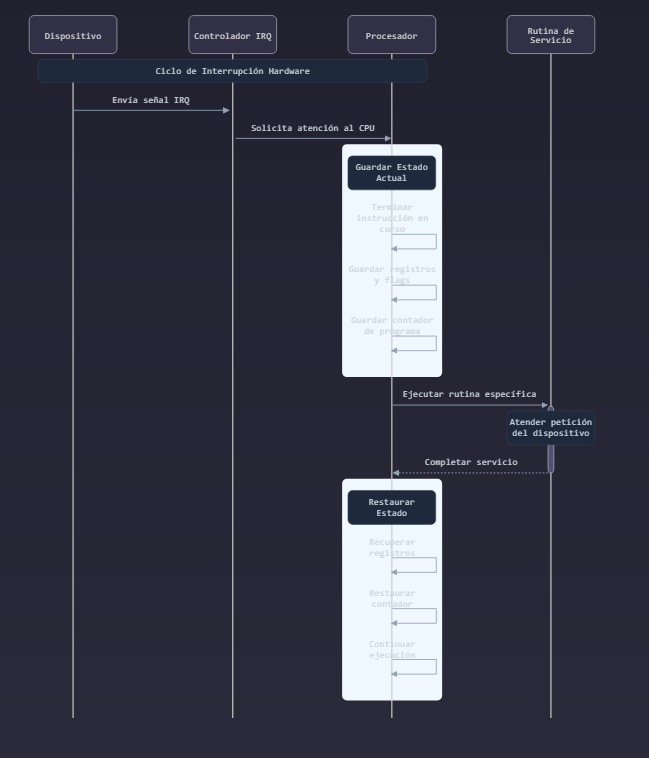
\includegraphics[width=10cm\textwidth]{figura_01_(practica04).png}
    \caption{Dispositivo, Controlador IRQ y Procesador}
    \label{fig:img1}
\end{figure}

\quad

\quad
\newpage






\section{¿Qué diferencias hay entre gestionar E/S con sondeo y hacerlo con interrupciones?}

\quad

{La gestión de Entrada/Salida (E/S) en computadoras puede realizarse principalmente de dos formas: mediante sondeo (polling) o mediante interrupciones. A continuación se mostrará un cuadro con las diferencias entre ambos métodos:}

\quad

\begin{tabular}{| p{3.5cm} |p{4cm} | p{4cm} |}
    \hline
    CARACTERÍSTICA & SONDEO (POLLING) & INTERRUPCIONES \\
    \hline
    Método & El procesador pregunta periódicamente a los dispositivos si necesitan atención. & Los dispositivos notifican al procesador cuando necesitan atención.
\\
    \hline
    Eficiencia & Muy ineficiente, consume recursos constantemente en preguntas innecesarias. & Altamente eficiente, el procesador solo actúa cuando es necesario. \\
    \hline
    Uso del CPU & Alto consumo de ciclos del procesador en preguntas repetitivas. & Libera al procesador para realizar otras tareas. \\
    \hline
    Complejidad & Implementación simple en hardware. & Requiere hardware adicional más complejo. \\
    \hline
    Latencia & Puede perder eventos si ocurren entre sondeos. & Responde inmediatamente a los eventos. \\
    \hline
    Aplicaciones típicas & Sistemas simples o con pocas operaciones de E/S. & Sistemas modernos multitarea y aplicaciones complejas.
 \\
    \hline

\end{tabular}\vspace{0.8cm}

{En los diagramas (rojo claro y verde claro) se podrá observar lo siguiente:}

\quad


\textbf{    •} { El diagrama rojo claro (lado izquierdo del cuadro) muestra cómo el procesador constantemente pregunta al dispositivo si necesita atención.}

\textbf{    •} { El diagrama verde claro (lado derecho del cuadro) ilustra cómo el procesador continúa con sus tareas mientras espera que el dispositivo lo interrumpa.}

\textbf{    •} { Las flechas indican el flujo de control y comunicación entre componentes.}

\begin{figure}[h]
    \centering
    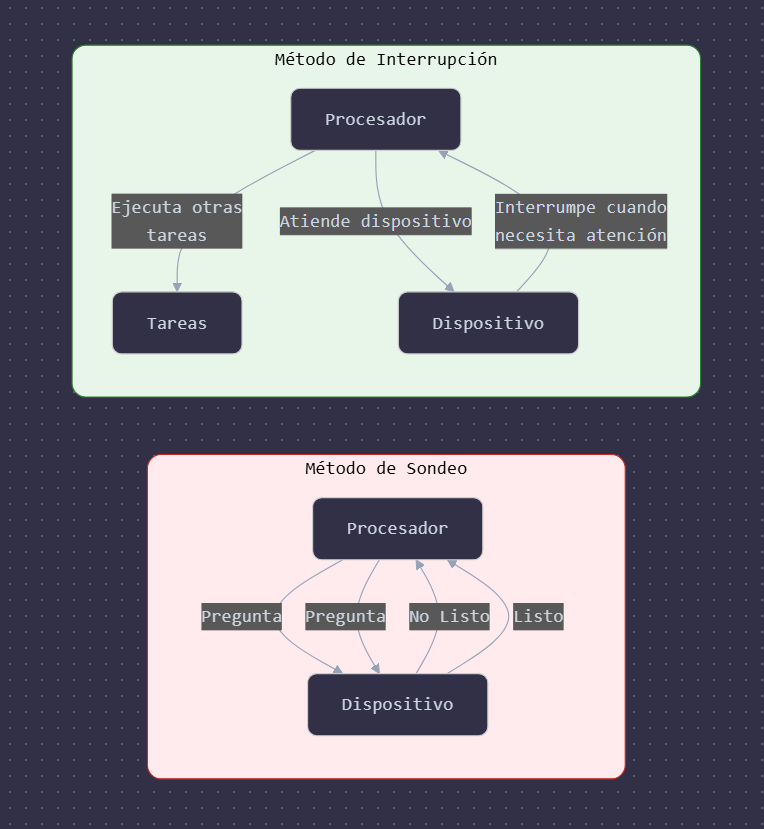
\includegraphics[width=10cm\textwidth]{figura_02_(practica04).png}
    \caption{Sondeo e Interrupciones}
    \label{fig:img1}
\end{figure}

\quad
\newpage
\quad
\newpage





\section{¿Qué ventajas tiene el uso de interrupciones en términos de uso del procesador?}

{Las interrupciones ofrecen varias ventajas significativas en términos de uso del procesador, que se pueden analizar detalladamente en el siguiente cuadro:}

\quad

\begin{tabular}{| p{3.5cm} |p{4cm} | p{4cm} |}
    \hline
    ASPECTO & VENTAJA & BENEFICIO PARA EL CPU \\
    \hline
    Eficiencia & El procesador solo actúa cuando es necesario. & Libera ciclos para otras tareas.\\
    \hline
    Gestión de tiempo & Permite ejecutar otras instrucciones mientras espera operaciones E/S. & Mayor rendimiento global del sistema. \\
    \hline
    Multitarea & Facilita la gestión simultánea de múltiples dispositivos. & Mejora la productividad del procesador. \\
    \hline
    Optimización & Evita el desperdicio de recursos en verificaciones innecesarias. & Reduce significativamente el consumo de ciclos. \\
    \hline

\end{tabular}\vspace{0.8cm}

\textbf{Impacto en el Rendimiento: }

\quad

{Las interrupciones mejoran significativamente el rendimiento del sistema porque:}

\quad

\textbf{    •} { Permiten una gestión eficiente de eventos asíncronos.}

\textbf{    •} { Evitan que el procesador pierda tiempo esperando a los dispositivos.}

\textbf{    •} { Mejoran la productividad global del sistema.}

\textbf{    •} { Facilitan la implementación efectiva de sistemas multitarea.}

\quad
\newpage





\section{¿Qué registros especiales se utilizan en MIPS32 para gestionar interrupciones?}

\quad

{En MIPS32, se utilizan varios registros especiales que trabajan en conjunto para gestionar eficientemente las interrupciones. Estos registros son fundamentales para el control y manejo de las interrupciones en el procesador.}

\quad

\textbf{Registros Esenciales en MIPS32 para Interrupciones: }

\quad

\textbf{{1 -  } {\underline{Registro Status - (\$12, CP0): }}}

\quad

\textbf{    •} { Controla el modo de operación del procesador.}

\textbf{    •} { Gestiona los niveles de prioridad.}

\textbf{    •} { Permite habilitar/deshabilitar interrupciones.}

\quad

\underline{Bits importantes: }

\quad

\textbf{    •} { IE (Bit 0): Interrupt Enable (1 = habilitadas, 0 = deshabilitadas).}

\textbf{    •} { EXL (Bit 1): Exception Level (1 = en excepción/interrupción, evita nuevas interrupciones).}

\textbf{    •} { IM (Bits 8–15): Interrupt Mask (habilita/deshabilita líneas de interrupción específicas).}

\textbf{    •} { UM (Bit 4): User Mode (0 = kernel, 1 = user).}



\quad

\textbf{{2 -  } {\underline{Registro Cause - (\$13, CP0)}}}

\quad

\textbf{    •} { Almacena información sobre la fuente de la interrupción.}

\textbf{    •} { Identifica el tipo de excepción o interrupción.}

\textbf{    •} { Ayuda en la priorización de interrupciones.}

\quad

\underline{Bits importantes: }

\quad

\textbf{    •} { IP (Bits 8–15): Interrupt Pending (muestra qué interrupciones están pendientes).}

\textbf{    •} { ExcCode (Bits 2–6): Exception Code (código del tipo de excepción, ej: 0 = interrupción hardware).}

\quad

\textbf{{3 -  } {\underline{Registro EPC (Exception Program Counter) - (\$14, CP0)}}}

\quad

\textbf{    •} { Guarda la dirección de la instrucción que se estaba ejecutando cuando ocurrió la interrupción (para retornar después).}

\textbf{    •} { Permite el retorno correcto después de atender la interrupción.}

\textbf{    •} { Mantiene el contexto del programa interrumpido.}

\quad

\textbf{{4 -  } {\underline{Registro BadVAddr (\$8, CP0)}}}

\quad

{Guarda la dirección de memoria que causó una excepción (ej: acceso inválido). No se usa en interrupciones simples.}

\quad

\textbf{{5 -  } {\underline{Registro Context (\$4, CP0)}}}

\quad

{Ayuda en el manejo de excepciones de memoria (como TLB misses), pero no es crítico para interrupciones básicas.}

\quad

\textbf{Ejemplo de Configuración de Interrupciones: }

\begin{figure}[h]
    \centering
    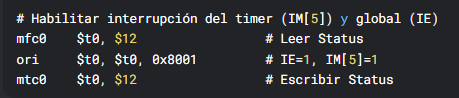
\includegraphics[width=10cm\textwidth]{figura_03_(practica04).png}
    \caption{Para Habilitar Interrupciones del Temporizador}
    \label{fig:img1}
\end{figure}


\quad
\newpage






\section{¿Por qué es necesario guardar el contexto (registros) al entrar en una rutina de servicio?}

\quad

{El guardado del contexto (registros) es una operación fundamental cuando se entra en una rutina de servicio de interrupción. A continuación se mostrarán algunas razones principales:}

\quad

\textbf{ Razones Principales: }

\quad

\textbf{1 -  } {\underline{Preservación del Estado del Programa: }}

\quad

\textbf{    •} { El programa principal estaba en plena ejecución cuando ocurrió la interrupción.}

\textbf{    •} { Los registros contenían valores importantes para esa ejecución.}

\textbf{    •} { Es necesario mantener estos valores para poder continuar correctamente después.}


\quad

\textbf{2 -  } {\underline{Independencia de Operaciones: }}

\quad

\textbf{    •} { La rutina de servicio necesita usar los registros para su propia ejecución.}

\textbf{    •} { Si no se guardaran, los valores del programa original se perderían.}

\textbf{    •} { Cada rutina de servicio puede necesitar diferentes registros.}

\quad

\textbf{Ejemplo Práctico: }

\quad

{Se considera el siguiente ejemplo simple:}

\begin{figure}[h]
    \centering
    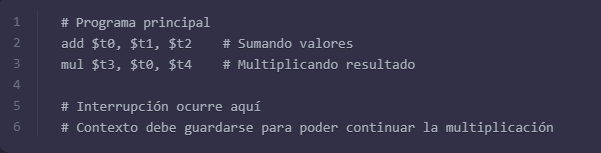
\includegraphics[width=10cm\textwidth]{figura_04_(practica04).png}
    \caption{Ejemplo con una Suma y una Multiplicación}
    \label{fig:img1}
\end{figure}

\quad

{Si no se guardara el contexto:}

\quad

\textbf{    •} { El valor de \$t0 (resultado de la suma) se perdería.}

\textbf{    •} { La multiplicación no podría completarse correctamente.}

\textbf{    •} { El programa principal produciría resultados incorrectos.}


\quad
\newpage








\section{Momentos en que pueden generarse excepciones en un sistema MIPS32}

\subsection*{a) Enumera al menos 4 situaciones en las que se pueda generar una excepción (por ejemplo: desbordamiento aritmético, fallo de dirección, etc.).}

\subsection*{b) Explica qué etapas del pipeline pueden provocar una excepción y por qué}

\quad

{Las excepciones en MIPS32 son eventos que alteran el flujo normal de ejecución del programa. Estos eventos pueden ocurrir en diferentes momentos y etapas del procesador.}

\quad

\textbf{ Situaciones que Generan Excepciones: }

\quad

\textbf{1 -  } {\underline{Desbordamiento Aritmético: }}

\quad

\textbf{    •} { Ocurre durante operaciones aritméticas que exceden el rango del registro.}

\textbf{    •} { Ejemplo: Suma de dos números positivos que resulta en un valor mayor que 2^31-1.}

\textbf{    •} { Se detecta en la etapa de ejecución (EX) del pipeline.}

\quad

\textbf{2 -  } {\underline{Fallo de dirección: }}

\quad

\textbf{    •} { Acceso a una dirección no alineada (ej: lw o sw en una dirección que no es múltiplo de 4).}

\textbf{    •} { Ejemplo: lw \$t0, 0x1001(\$zero) (0x1001 no es múltiplo de 4)..}

\quad

\textbf{3 -  } {\underline{Acceso a Memoria Inválido: }}

\quad

\textbf{    •} { Se genera al intentar acceder a direcciones no mapeadas.}

\textbf{    •} { Ocurre durante la etapa de memoria (MEM).}

\textbf{    •} { Incluye violaciones de segmento y páginas no presentes.}

\quad

\textbf{4 -  } {\underline{Instrucción No Valida: }}

\quad

\textbf{    •} { Se produce al decodificar una instrucción ilegal.}

\textbf{    •} { Detectada en la etapa de decodificación (ID).}

\textbf{    •} { Incluye códigos de operación inválidos.}

\quad

\textbf{5 -  } {\underline{División por Cero: }}

\quad

\textbf{    •} { Ocurre durante operaciones de división.}

\textbf{    •} { Se detecta en la etapa de ejecución (EX).}

\textbf{    •} { Es una excepción aritmética crítica.}

\quad

\textbf{ Etapas del Pipeline que Pueden Producir Excepciones: }

\quad

\textbf{1 -  } {\underline{Etapa IF (Instruction Fetch - Búsqueda de Instrucción): }}

\quad

\textbf{    •} { Puede detectar instrucciones ilegales en la memoria.}

\textbf{    •} { Se produce cuando el código de operación no es válido.}

\textbf{    •} { La detección ocurre antes de la decodificación completa.}

\quad

\textbf{2 -  } {\underline{Etapa ID (Decode - Decodificación): }}

\quad

\textbf{    •} { Detecta instrucciones no válidas después de la decodificación.}

\textbf{    •} { Verifica permisos de acceso a registros.}

\textbf{    •} { Identifica operaciones no permitidas en el modo actual.}

\quad

\textbf{3 -  } {\underline{Etapa EX (Execute - Ejecutar): }}

\quad

\textbf{    •} { Es la etapa más propensa a excepciones.}

\textbf{    •} { Detecta desbordamientos aritméticos.}

\textbf{    •} { Identifica divisiones por cero.}

\textbf{    •} { Verifica operaciones no permitidas.}

\quad

\textbf{4 -  } {\underline{Etapa MEM (Memory Access - Acceso a Memoria)): }}

\quad

\textbf{    •} { Detecta fallos de alineación.}

\textbf{    •} { Identifica violaciones de segmento.}

\textbf{    •} { Verifica accesos a memoria inválidos.}

\quad

\textbf{5 -  } {\underline{WB (Write Back - Escritura Diferida): }}

\quad

\textbf{    •} { En MIPS32, esta etapa no genera excepciones, ya que los errores se detectan en etapas anteriores (MEM o EX).}

\quad

{En el diagrama se puede observar:}

\quad

\textbf{    •} { Las flechas muestran el flujo normal del pipeline (arriba) y los puntos de detección de excepciones (centro).}

\textbf{    •} { Cada etapa puede generar diferentes tipos de excepciones.}

\textbf{    •} { El proceso de manejo de excepciones (abajo) es común para todas las excepciones detectadas.}

\quad


\begin{figure}[h]
    \centering
    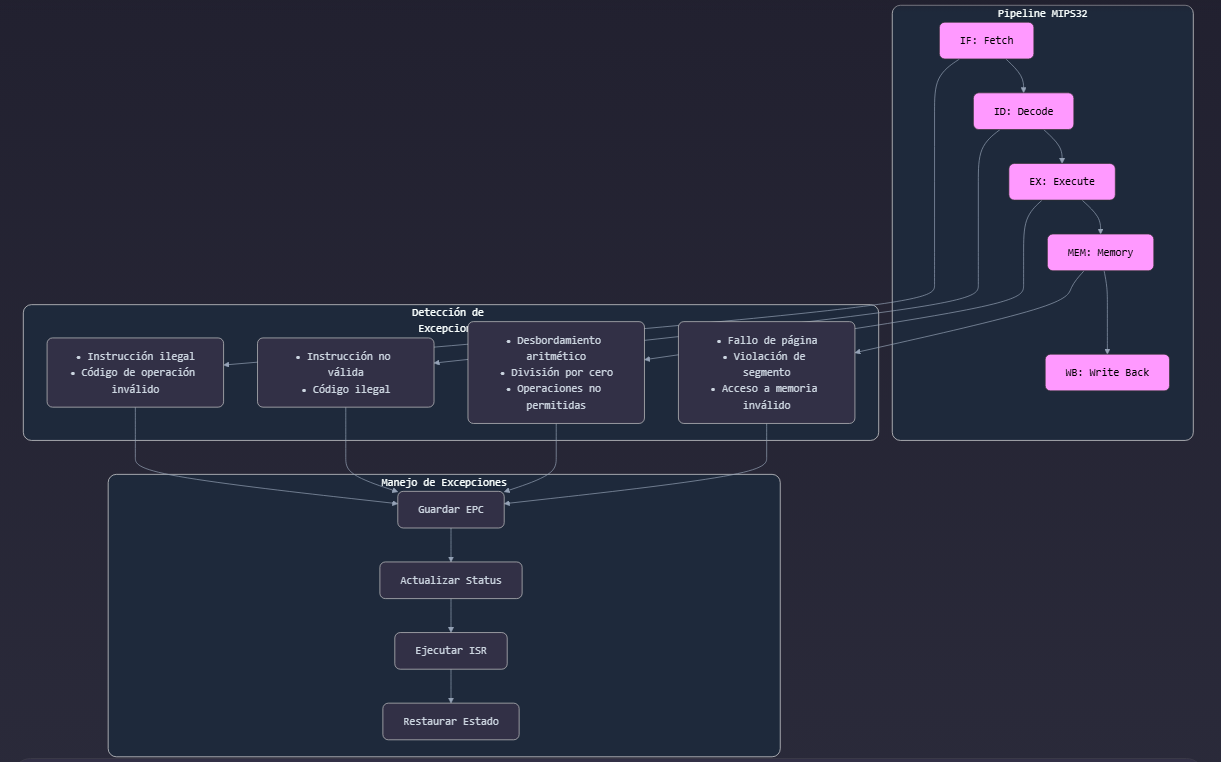
\includegraphics[width=10cm\textwidth]{figura_05_(practica04).png}
    \caption{Etapas del Pipeline que Pueden Producir Excepciones}
    \label{fig:img1}
\end{figure}


\quad
\newpage
\quad
\newpage







\section{Estrategias de tratamiento de excepciones e interrupciones}

\subsection*{a) Explica las diferencias entre interrupciones y excepciones (¿son síncronas o asíncronas?).}

\subsection*{b) Describe brevemente dos estrategias para tratar excepciones en un sistema MIPS32 ¿Cómo se redirige la ejecución hacia la rutina de servicio? ¿Cuál es la función del registro EPC (Exception Program Counter)?}

\quad

{Las interrupciones y excepciones son mecanismos muy importantes para el rendimiento de los sistemas informáticos. Su correcta gestión, en gran medida a cargo del sistema operativo, es lo que permite que los programas de software convivan con el hardware y reaccionen de forma controlada a eventos inesperados, por eso primero se va a profundizar en las diferencias entre interrupciones y excepciones:}

\quad

\begin{table}[h!]

    \label{tab:diff_excepciones_interrupciones}
    \begin{tabularx}{\textwidth}{p{2cm} >{\raggedright\arraybackslash}X >{\raggedright\arraybackslash}X}
    \toprule
    \textbf{Característica} & \textbf{Interrupción} & \textbf{Excepción} \\
    \midrule
    \textbf{Causa} & Es un evento externo a la CPU. & Es un evento interno a la CPU, causado por la ejecución de una instrucción. \\
    \midrule
    \textbf{Sincronicidad}& \textbf{Asíncrona.} Puede ocurrir en cualquier momento, independientemente del programa que se esté ejecutando en la CPU. & \textbf{Síncrona.} Siempre ocurre como resultado directo de una instrucción en particular que se está ejecutando en ese momento. \\
    \midrule
    \textbf{Ejemplos} & • Un temporizador de hardware que expira. \newline • Un dispositivo de E/S que termina una operación (teclado, disco duro, red). & • División por cero. \newline • Acceso a una dirección de memoria no válida (violación de segmento). \newline • Una instrucción ilegal. \\
    \midrule
    \textbf{Propósito} & Notificar a la CPU sobre eventos externos para que pueda realizar una acción. & Indicar un error o una condición excepcional que el programa no puede manejar por sí mismo. \\
    \midrule
    \textbf{Tipos} & Por hardware (E/S, temporizador) y por software (llamadas al sistema). & Fallos, trampas y abortos. \\
    \midrule
    \textbf{Recuperación} & El sistema operativo atiende la interrupción y, por lo general, el programa original puede reanudarse sin problemas. & Su recuperación puede implicar corregir el error y continuar, pero a menudo resulta en la terminación del proceso. \\
    \bottomrule
    \end{tabularx}
\end{table}
\newpage

\quad

\textbf{Estrategias de Tratamiento de Excepciones en MIPS32}

\quad

\textbf{1.   }{\underline{Uso del Vector de Inicio (BEV=1):}{Esta es la estrategia por defecto, especialmente al iniciar el sistema o en sistemas muy simples. Cuando el bit BEV en el registro Status es 1, todas las excepciones (tanto interrupciones de hardware como excepciones de software) son redirigidas a una única dirección de memoria fija: 0xBFC00200}

\quad

\textbf{2.   }{\underline{Uso del Vector General (BEV=0):}{Esta es la estrategia utilizada por los sistemas operativos modernos. Cuando el bit BEV es 0, las excepciones son redirigidas a una dirección de memoria diferente: 0x80000080. Además, algunas excepciones específicas (como interrupciones o fallos de dirección) pueden ser redirigidas a un vector secundario, lo que agiliza el proceso.}


\quad

\textbf{Explicación de como se redirije la ejecución hacia la rutina de servicio}

\quad

\textbf{1.   }{El procesador detecta una condición de excepción.}

\quad

\textbf{2.   }{El hardware automáticamente guarda el valor del contador de programa (PC) actual en el registro EPC (Exception Program Counter).}

\quad

\textbf{3.   }{El hardware escribe un código de excepción (ExcCode) en el registro Cause para indicar la razón de la excepción.}

\quad

\textbf{4.   }{El hardware modifica el registro Status, típicamente estableciendo el bit ExL (Exception Level) a 1. Esto deshabilita las interrupciones y eleva los privilegios del procesador al modo kernel.}

\quad

\textbf{5.   }{El hardware carga en el contador de programa (PC) la dirección de memoria de la rutina de servicio de excepciones. Esta dirección es 0xBFC00200 o 0x80000080, dependiendo del estado del bit BEV}

\quad

\textbf{6.   }{El procesador comienza a ejecutar el código de la rutina de servicio de excepciones.}

\quad
\newpage


\textbf{¿Cuál es la función del registro EPC (Exception Program Counter)?}

\quad

{Su función principal es almacenar la dirección de memoria de la instrucción donde ocurrió la excepción, o la dirección de la siguiente instrucción, para que el sistema pueda retomar la ejecución del programa una vez que la excepción ha sido manejada.}

\quad

{Para fallos de una intrucion, el EPC guardara la dirección de la instrucción que intentó acceder a una página de memoria no presente. El manejador de excepciones carga la página en memoria y luego regresa al programa usando la instrucción eret. El procesador utiliza el valor de EPC para volver a ejecutar la instrucción que falló, la cual ahora tendrá éxito.}

\quad

{Para las execciones intencionadas, (trampas) el EPC guardara la dirección de la instrucción syscall. El manejador de excepciones realiza el servicio solicitado. Para regresar, el manejador de excepciones debe incrementar el valor de EPC en 4 bytes (el tamaño de una instrucción) antes de ejecutar eret. Esto es crucial para que la ejecución se reanude después de la instrucción syscall, y no vuelva a ejecutarla en un bucle infinito.}

\quad
\newpage







\section{Habilitación de interrupciones en dispositivos y procesador}

\subsection*{a) Explica cómo se habilitan las interrupciones en:}
\subsubsection*{El teclado.}
\subsubsection*{La pantalla.}
\subsubsection*{El procesador (detalla qué bits del registro Status deben modificarse).}

\subsection*{b) ¿Qué pasaría si habilitamos interrupciones en los dispositivos, pero no en el procesador?}

\quad

{Algunas de las interrupciones de las que se va a hablar a continuación (Teclado y pantalla) son nivel de hardware, es decir que además de depender del software (El procesador), dependen de un periférico con controlador inicializado y una conexión a la línea IRQ, así podrá generar interrupciones.}

\subsection{Interrupción por Teclado}
\begin{itemize}
    \item \textbf{A nivel de Hardware:}
    \begin{itemize}
        \item El controlador del teclado tiene un búfer para las teclas presionadas.
        \item Cuando una tecla es presionada el búfer tiene datos disponibles, el controlador genera una señal eléctrica en una de las líneas IRQ del sistema.
    \end{itemize}
    \item \textbf{A nivel de Software:}
    \begin{itemize}
        \item Se debe habilitar la interrupción IM0 en el registro Status del procesador MIPS32.
        \item Cuando el procesador detecta la interrupción, salta a la rutina de servicio de interrupción (ISR) del teclado.
        \item La ISR lee el carácter del búfer del teclado, lo procesa y luego borra la señal de interrupción en el controlador del teclado.
         \item Finalmente, la ISR retorna, y el procesador retoma el programa que fue interrumpido.

    \end{itemize}
\end{itemize}

\subsection{Interrupción por Pantalla (Display)}
\begin{itemize}
    \item \textbf{A nivel de Hardware:}
    \begin{itemize}
        \item Se puede usar un controlador de video (Sincronización vertical) genera una interrupción cuando el rayo de electrones (en monitores antiguos) o el barrido del framebuffer (en pantallas modernas) llega al final de la pantalla y se prepara para el siguiente cuadro.
        \item Una interrupción puede señalizar que una operación de dibujo compleja (ej. mover un bloque de memoria a la pantalla) ha finalizado.
    \end{itemize}
    \item \textbf{A nivel de Software:}
    \begin{itemize}
        \item El sistema operativo habilita la interrupción correspondiente a la línea IRQ del controlador de video.
        \item La ISR del controlador de video se encarga de manejar el evento, como actualizar el buffer de la pantalla o notificar a un proceso de usuario que el dibujo ha terminado.
    \end{itemize}
\end{itemize}


\subsection{Interrupción por Procesador (Propiamente dicha):}
\begin{itemize}
    \item \textbf{A nivel de Hardware:}
    \begin{itemize}
        \item El procesador establece el bit  ExL en 1 cuando entra en un manejador de excepción, de esta forma todas las interrupciones externas (hardware) son deshabilitadas, incluso si el bit IEc está habilitado. Esto evita que una interrupción externa interrumpa la ejecución del manejador de excepción, lo que podría llevar a un estado inconsistente.
        \item ExL también puede cambiar el modo de operación de la CPU a modo kernel (modo privilegiado), lo que permite al manejador de excepción acceder a recursos protegidos.
        \item Es importante distinguir entre ExL y ERL. ExL se usa para excepciones "normales" de las que se espera regresar (como una syscall o un page fault). ERL se usa para errores graves e irrecuperables, como un reset, una NMI (interrupción no-mascarable) o un error de caché. Cuando ERL es 1, el procesador también está en modo kernel con las interrupciones deshabilitadas.
    \end{itemize}
    \item \textbf{A nivel de Software:}
    \begin{itemize}
        \item Aunque el hardware ya ha deshabilitado las interrupciones al establecer ExL, el manejador de excepción podría querer habilitarlas de nuevo en un punto seguro de su ejecución para poder atender interrupciones anidadas si la arquitectura lo permite, o para evitar un bloqueo del sistema. Esto se haría modificando el bit IEc (Interrupt Enable) y la máscara de interrupciones (IM). Esta instrucción genera una excepción interna en el procesador.
        \item Cuando el manejador de excepción termina su trabajo, debe restaurar el estado del procesador para que el programa original pueda reanudar su ejecución. Para ello, se usa la instrucción eret (return from exception). La instrucción eret restaura automáticamente el valor de Status y el contador de programa (EPC) guardado para la excepción, lo que, entre otras cosas, limpia el bit ExL para reanudar el estado normal de interrupciones. Esta
    \end{itemize}
\end{itemize}


\subsection{¿que pasaria si habilitamos interrupciones en los dispositivos, pero no en el procesador?}

{Si las interrupciones se habilitan en los dispositivos, pero no en el procesador, los dispositivos periféricos seguirán enviando señales eléctricas de interrupción (peticiones IRQ) al procesador cuando un evento ocurra, como al presionar una tecla o al terminar una operación de E/S.}

\quad

{Sin embargo, el procesador no las reconocerá ni las atenderá. Esto se debe a que, para que el procesador pueda responder a una interrupción, el bit de habilitación de interrupciones (IEc) en su registro Status debe estar activo. Si este bit está deshabilitado, el procesador ignorará las señales de interrupción que reciba de los dispositivos externos, sin importar si los dispositivos las están generando correctamente o no.}

\quad

{En resumen, la habilitación de interrupciones en los dispositivos es solo una parte del proceso; la habilitación a nivel de procesador es la que permite que el sistema responda y gestione las peticiones de interrupción de manera efectiva.}

\quad
\newpage









\section{Procesamiento de interrupciones}

\subsection*{a) Describe paso a paso qué ocurre cuando se produce una interrupción de reloj:}
\subsubsection*{Desde que el evento ocurre hasta que la rutina de servicio termina.}
\subsubsection*{¿Qué registros se guardan y restauran?}
\subsubsection*{¿Qué hace el hardware y qué hace el software (sistema operativo o rutina)?}

\subsection*{b) ¿Por qué es importante guardar el contexto (registros generales, EPC, Status) al entrar en la rutina?}

\quad

\textbf{Paso a Paso: Ciclo de una Interrupción de Reloj}

\quad

\subsection{ Generación de la Señal de Interrupción (Hardware)}
\begin{enumerate}
    \item \textbf{Evento:} Un contador de hardware, integrado en un chip temporizador, alcanza un valor predefinido.
    \item \textbf{Acción del Hardware:} El temporizador genera una señal eléctrica, una \textbf{petición de interrupción (IRQ)}, que envía a una de las líneas de interrupción del procesador. En la arquitectura MIPS32, esta suele ser la interrupción de hardware número 7 (\texttt{IP7}), reservada para el temporizador.
\end{enumerate}

\subsection{ Detección y Preparación por la CPU (Hardware)}
\begin{enumerate}
    \item \textbf{Detección:} Al final de la ejecución de una instrucción, el procesador verifica si hay interrupciones pendientes y si están habilitadas (\texttt{IEc} en el registro \texttt{Status} es 1) y enmascaradas correctamente (\texttt{IM7} en el registro \texttt{Status} es 1).
    \item \textbf{Guardado del estado del programa:} El procesador realiza las siguientes acciones automáticas:
    \begin{itemize}
        \item Guarda el valor actual del \textbf{contador de programa (PC)} en el registro \textbf{\texttt{EPC}} (Exception Program Counter).
        \item Modifica el registro \texttt{Status} del Coprocesador 0, estableciendo el bit \textbf{\texttt{ExL} a 1}, lo que deshabilita inmediatamente las interrupciones anidadas.
    \end{itemize}
\end{enumerate}

\subsection{ Redirección al Manejador (Hardware)}
\begin{enumerate}
    \item \textbf{Búsqueda del manejador:} El hardware consulta la tabla de vectores de excepciones para encontrar la dirección de memoria de la rutina de servicio.
    \item \textbf{Salto:} El procesador carga la dirección del manejador de interrupciones en el contador de programa (PC), transfiriendo el control a la rutina de servicio del reloj.
\end{enumerate}

\subsection{ Ejecución de la Rutina de Servicio (Software del Sistema Operativo)}
\begin{enumerate}
    \item \textbf{Identificación de la interrupción:} El manejador de excepciones del sistema operativo lee el registro \texttt{Cause} y su campo \texttt{ExcCode} para confirmar que se trata de la interrupción del temporizador (\texttt{IP7}).
    \item \textbf{Guardado de contexto del proceso:} El kernel guarda todos los registros de propósito general, registros de punto flotante, etc., del proceso que fue interrumpido en su \textbf{Bloque de Control de Proceso (PCB)}.
    \item \textbf{Atención al temporizador:} El manejador realiza sus tareas:
    \begin{itemize}
        \item Actualiza la "hora" del sistema.
        \item Decrementa el contador de tiempo restante del proceso actual (su \textit{quantum}).
        \item Vuelve a programar el temporizador para la próxima interrupción.
    \end{itemize}
    \item \textbf{Planificación (Scheduling):} El kernel verifica si el proceso actual ha agotado su \textit{quantum} de tiempo. Si lo ha hecho, el planificador elige otro proceso de la cola de "listos" para que se ejecute.
    \item \textbf{Restauración de contexto del nuevo proceso:} El kernel carga los registros de contexto del nuevo proceso (o del mismo si no hubo cambio), incluyendo su contador de programa (\texttt{PC}).
\end{enumerate}

\subsection{ Fin de la Rutina de Servicio y Retorno}
\begin{enumerate}
    \item \textbf{Restauración del EPC:} El manejador de excepciones del kernel carga en el registro \texttt{EPC} la dirección donde debe continuar la ejecución del nuevo proceso (o del anterior).
    \item \textbf{Instrucción \texttt{eret}:} El manejador ejecuta la instrucción \textbf{\texttt{eret}} (Return from Exception), la cual realiza las siguientes acciones:
    \begin{itemize}
        \item Carga el valor de \texttt{EPC} en el contador de programa (PC).
        \item Restaura el valor original del registro \texttt{Status}, lo que \textbf{limpia el bit \texttt{ExL}} y rehabilita las interrupciones.
    \end{itemize}
\end{enumerate}

\subsection{ Reanudación de la Ejecución del Programa}
El procesador comienza a ejecutar el nuevo proceso (o el mismo proceso que fue interrumpido) como si nada hubiera pasado. Las interrupciones vuelven a estar habilitadas, y el ciclo continúa.

\quad
\newpage
\textbf{Importancia de guardar el contexto(registros generales,EPC,STAUS) al entrar a una rutina}

\quad

\textbf{1.   } \underline{Registros de propósito general:}  {Guardar estos registros es vital para preservar los datos y variables con los que el programa estaba trabajando.}
\quad

\textbf{2.   } \underline{Registro EPC:}  {Guardar estos registros es vital para preservar los datos y variables con los que el programa estaba trabajando.}
\quad

\textbf{3.   } \underline{Registro Status:}  {Crítico para el "cómo" volver a ejecutar. Preserva el estado de los bits de control del procesador (habilidad de interrupciones, modo de operación, etc.).}


\quad
\newpage







 \section{Interrupciones de reloj y control de ejecución}

\subsection*{a) Explica cómo una interrupción de reloj puede usarse para:}
\subsubsection*{Evitar que un programa quede en un bucle infinito.}
\subsubsection*{Finalizar programas que superan un tiempo máximo de ejecución.}

\subsection*{b) ¿Qué debe hacer el software si el programa finaliza antes de que ocurra la interrupción de reloj?}


\subsection{ Explicación de  cómo una interrupción de reloj puede usarse para:}

\subsubsection*{Evitar que un programa quede en un bucle infinito.}
\begin{itemize}
    \item La interrupción de reloj permite la implementación de la \textbf{multitarea preventiva}. El sistema operativo configura un temporizador de hardware para generar una interrupción a intervalos regulares, por ejemplo, cada 10 milisegundos.
    \item Cada vez que ocurre esta interrupción, el control de la CPU se transfiere forzosamente al kernel del sistema operativo.
    \item El kernel, al detectar la interrupción, puede examinar el estado del programa que se estaba ejecutando. Si el mismo programa ha estado usando el procesador por un tiempo excesivamente largo (sin ceder el control), el kernel puede detectar que está "atascado" en un bucle infinito y tomar medidas, como terminar el proceso o asignarle un tiempo de ejecución más corto.
    \item De esta forma, ningún programa puede monopolizar la CPU indefinidamente, lo que evita que el sistema se cuelgue.
\end{itemize}

\subsubsection*{Finalizar programas que superan un tiempo máximo de ejecución.}
\begin{itemize}
    \item Esta es una aplicación directa del mismo mecanismo de interrupción. Cuando un programa se inicia, el sistema operativo le asigna lapso de tiempo de CPU.
    \item El temporizador de hardware se configura para que genere una interrupción al expirar este lapso de tiempo de CPU.
    \item Si un programa excede el tiempo asignado (es decir, no ha terminado antes de que ocurra la interrupción), el manejador de interrupciones del reloj se activa.
    \item En ese momento, el kernel sabe que el programa ha agotado su tiempo. La rutina de servicio del reloj, a través de su planificador, guarda el estado del programa actual, lo marca como "listo" y elige otro programa para darle el control de la CPU.
    \item Si el tiempo máximo de ejecución de un programa se define como el total de sus lapsos de tiempo de CPU  asignados, el sistema operativo puede decidir finalizar el programa en lugar de volver a ponerlo en la cola de "listos".
\end{itemize}

\subsection{¿Qué debe hacer el software si el programa finaliza antes de que ocurra la interrupción de reloj?}

Si un programa finaliza por sí mismo (por ejemplo, mediante una llamada al sistema \texttt{exit}) antes de que se genere la interrupción de reloj programada, el software del sistema operativo debe realizar las siguientes acciones para gestionar la situación correctamente:

\begin{enumerate}
    \item \textbf{Detectar la finalización:} El programa ejecutará una llamada al sistema (\textit{syscall}) para solicitar su terminación. Esta \textit{syscall} genera una excepción de software que transfiere el control al kernel.
    \item \textbf{Cancelar la interrupción de reloj:} El kernel, al procesar la llamada de terminación, debe \textbf{desactivar proactivamente la interrupción de reloj pendiente} para ese proceso. Si no lo hiciera, la interrupción ocurriría de todos modos y sería espuria, ya que el proceso al que estaba asignado el \textit{quantum} ya no existe. Esto podría llevar a un estado inconsistente en el planificador.
    \item \textbf{Liberar recursos:} El sistema operativo lleva a cabo la limpieza del proceso. Esto incluye liberar la memoria, los archivos abiertos y otros recursos que el programa estaba utilizando.
    \item \textbf{Seleccionar un nuevo proceso:} El planificador del sistema operativo selecciona inmediatamente otro proceso de la cola de "listos" para que se ejecute, sin tener que esperar a la interrupción del temporizador.
\end{enumerate}


\quad
\newpage




\section{ Análisis y Discusión de los Resultados.}

\quad

{Podemos concluir que una interrupción de hardware permite que los dispositivos externos puedan solicitar la atención de la CPU de manera eficiente, sin necesidad de que la CPU esté constantemente verificando el estado de cada dispositivo. El ciclo de interrupción garantiza que las tareas importantes no se pierdan y que los dispositivos puedan recibir la atención necesaria de forma oportuna.}

\quad

{Es importante es conocer las caracteristicas de las interrupciones y las excepciones, ambos son mecanismos para el rendimiento de sistemas informaticos, pero muy distintos entre sí, mientras que las interrupciones son eventos externos al computador, que por lo general utilizan hardware como lo puede ser el teclado y que tienen generalmente un ciclo de reloj, las excepciones son eventos internos del CPU involuntarios que terminan con el programa que se esté realizando, por ello es que existen estrategias de prevención de exenciones.}

\quad

{Hay que mencionar que la correcta gestión de interrupciones depende de guardar y restaurar el contexto del programa, incluyendo los registros de propósito general, el registro Status y el registro EPC, el cual es un registro fundamental porque almacena la dirección de la instrucción donde ocurrió la excepción, lo que permite al sistema volver al punto correcto del programa una vez que se ha manejado el.}

\quad

\end{document}